\chapter{VBTE}
Nedenfor følger design af software til VBTE. Dette er lavet på baggrund af kravspecifikation og systemarkitektur. Bemærk der i dette design dokument blandt andet ikke er beskrevet mixer, pga osv. da deres eneste funktion er "Start();". Derudover er der en betydelig hardware del knyttet til dette modul, der refereres derfor til detaljeret hardware design for yderligere detaljer om VBTE modulet.
\section{Modulets ansvar}
Som beskrevet i systemarkitektur står VBTE'en for at måle vandniveauet i ballasttankene samt at lukke vand ind eller ud af ballasttankene. Hertil er der også en kommunikation med SM modulet indeholende instruktioner.
\section{Klassediagram}
Nedenfor ses klassediagrammet for VBTE. Bemærk at koden dog er i C men for overblikket er der lavet klassediagram.
\begin{figure}
\centering
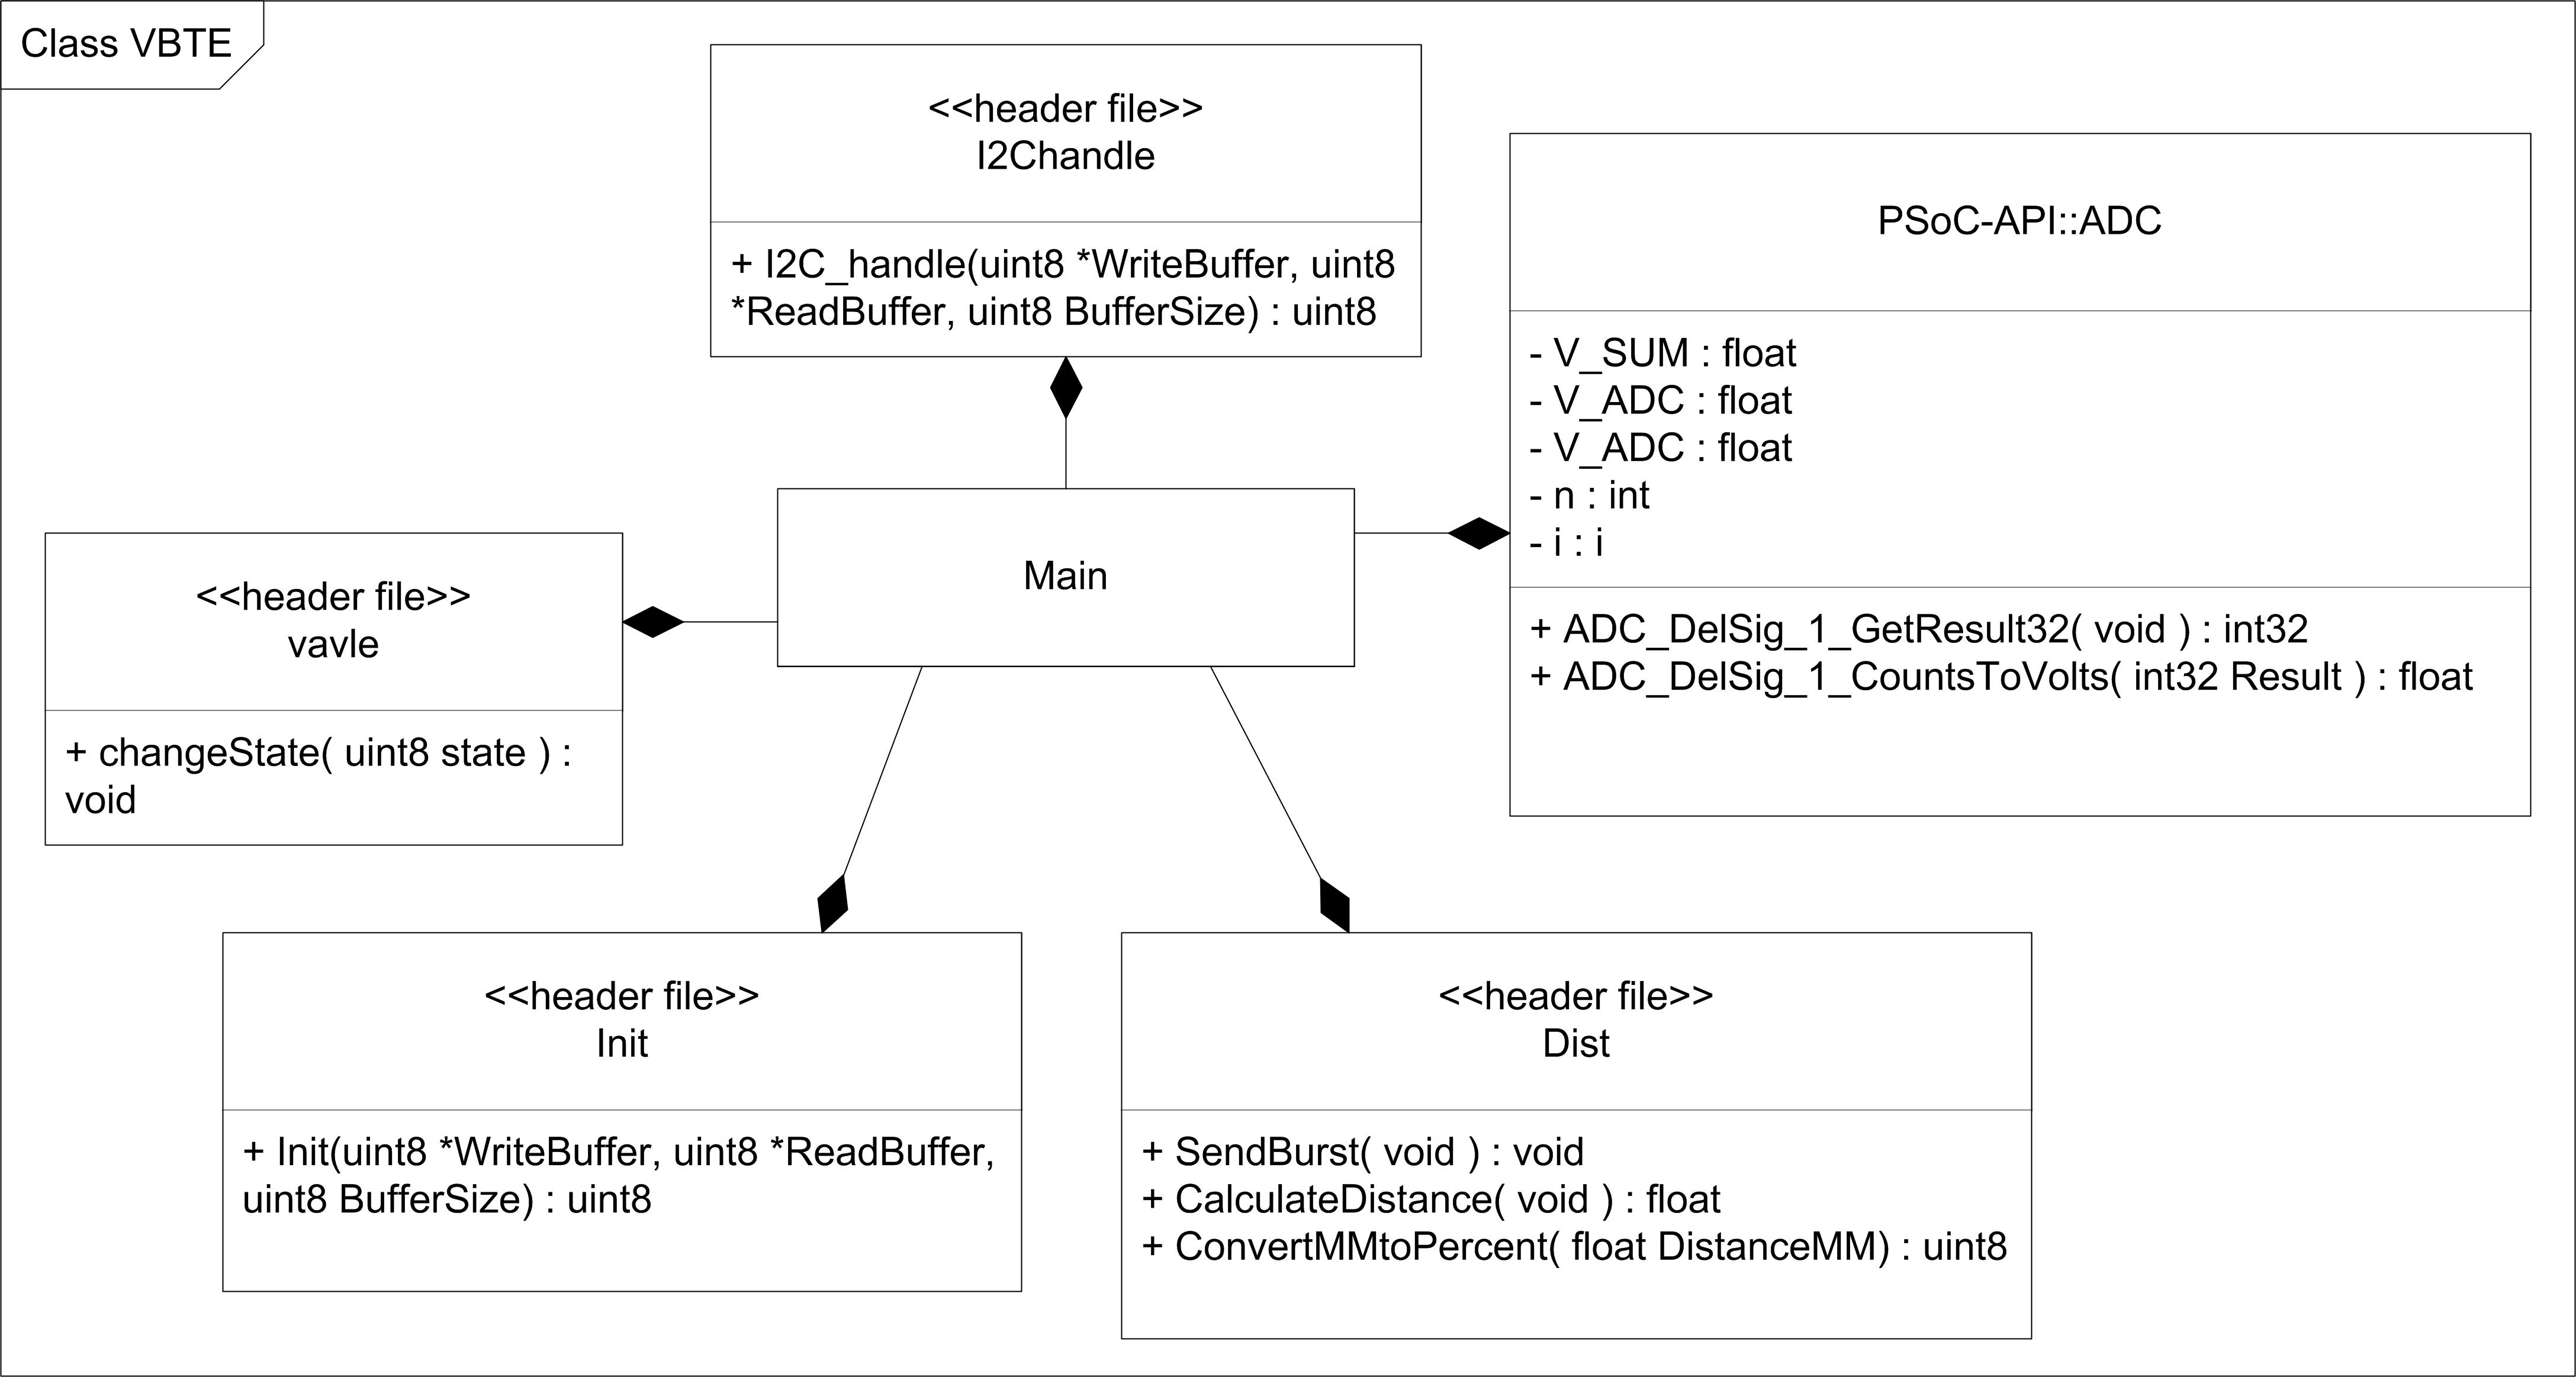
\includegraphics[width=1\textwidth]{billeder/ClassVBTE}
\caption{På figuren ses klassediagrammet for VBTE \textbf{Billedet skal opdateres}}
\end{figure}

\section{Globale variabler}
\begin{table}[H]
\begin{tabular}{|l|p{10cm}|}
\hline
\cellcolor[gray]{0.8}\textbf{Variabel} &\cellcolor[gray]{0.8} \textbf{Beskrivelse}\\ \hline
BurstLengthVal & Denne variabel er anvendt til at håndtere antallet af perioder burstet bliver sendt med.\\ \hline
WaitBurstVar & Bliver brugt til nonblocking delay til SendBurst funktionen.\\ \hline
BurstTimerVal & Holder på Timerens værdi når et burst er sendt.\\ \hline
DistanceTimerVal & Holder værdien på timeren når et burst er modtaget. \\ \hline
CalcDistFlag & Bliver sat når et burst er modtaget så en afstand kan blive beregnet.\\ \hline
\end{tabular}
\end{table}
\section{Metode- og klassebeskrivelser}
\subsection{Valve}
\subsubsection{Ansvar}
Denne header har til ansvar at styre ventilerne ud fra "state"-variablen modtaget fra I2C\_handle. Headeren benytter PSoC-API'et til kontrol registre..
\subsubsection{Funktionsbeskrivelser}
 
\begin{table}[H]
\begin{tabular}{l p{12.5cm}}
\multicolumn{2}{l}{\textcolor{blue}{void} ChangeState( \textcolor{blue}{uint8} state );} \\
\hline
Beskrivelse:& Funktionen anvender API'et fra I2C blokken i PSoC miljøet. Med disse tjekker den om der er fyldt nyt i bufferen og aflæse dette. Herfer kalder den funktionen I2C\_decode(); til at afkode beskeden fra SM. Herefter klargøres readbufferen til evt. at sende vandniveau tilbage. \\
Parametre:&\textcolor{blue}{uint8}* WriteBuffer\\
&\textcolor{blue}{uint8}* ReadBuffer\\
&\textcolor{blue}{uint8} BufferSize \\
Returværdi:& \textcolor{blue}{uint8} State\\
\end{tabular}
\end{table}

\subsection{Dist}
\subsubsection{Ansvar}
Denne header har til ansvar at sende burst, beregne afstanden samt at omregne afstanden til procent.
\subsubsection{Funktionsbeskrivelser}

\begin{table}[H]
\begin{tabular}{l p{12.5cm}}
\multicolumn{2}{l}{\textcolor{blue}{void} SendBurst( \textcolor{blue}{void} );} \\
\hline
Beskrivelse:&Denne metode aktiverer en 40kHz clock og tæller perioderne op til 10, lukker for burstet og ligger timerens værdi ind i den globale variabel BurstTimerVal\\
Parametre:&Ingen\\
Returværdi:&Ingen\\
\end{tabular}
\end{table}

\begin{table}[H]
\begin{tabular}{l p{12.5cm}}
\multicolumn{2}{l}{\textcolor{blue}{float} CalculateDistance( \textcolor{blue}{void} );} \\
\hline
Beskrivelse:&Denne metode anvender BurstTimerVal og DistanceTimerVal til at finde ud af hvor mange clocks der er gået fra burstet er blevet sendt til det igen er blevet registreret.\\
Parametre:&Ingen\\
Returværdi:&Afstanden i MM (fra tankbunden til vandniveauet\\
\end{tabular}
\end{table}

\begin{table}[H]
\begin{tabular}{l p{12.5cm}}
\multicolumn{2}{l}{\textcolor{blue}{uint8} ConvertMMtoPercent( \textcolor{blue}{float} );} \\
\hline
Beskrivelse:&Denne metode aktiverer en 40kHz clock og tæller perioderne op til 10, lukker for burstet og ligger timerens værdi ind i den globale variabel BurstTimerVal\\
Parametre:&Ingen\\
Returværdi:&Ingen\\
\end{tabular}
\end{table}
\subsection{Eventuelle Sekvensdiagrammer og state machines}
hab hab